\chapter{Introducción}

En el escenario del desarrollo de software e infraestructura moderna, el uso de contenedores se ha consolidado como una estrategia clave para resolver los problemas clásicos de inconsistencia de entornos y facilitar el despliegue de aplicaciones. El presente informe técnico detalla el proceso de diseño e implementación de un stack web dinámico utilizando Docker, desarrollado en el marco del Laboratorio Práctico N°2. El propósito central de esta experiencia práctica consiste en desplegar una aplicación web funcional capaz de realizar las cuatro operaciones esenciales de gestión de datos (CRUD: Crear, Leer, Actualizar y Borrar) dentro de un ecosistemaF controlado y seguro.\\
\\
Para dar cumplimiento a los requisitos técnicos establecidos, la arquitectura se estructuró mediante la herramienta \texttt{docker-compose}, dividiendo el sistema en dos microservicios principales: un contenedor para la aplicación web configurado mediante un archivo \texttt{Dockerfile} personalizado (PHP) y un contenedor para el motor de base de datos relacional utilizando una imagen oficial (MariaDB). A lo largo de este documento, se expondrá la evidencia técnica del despliegue, analizando aspectos críticos de la infraestructura como el aislamiento de los servicios dentro de una red virtual privada de Docker y la configuración de volúmenes para garantizar la persistencia de los datos de forma independiente al ciclo de vida de los contenedores.

\chapter{Desarrollo}
A continuación, se presenta la evidencia técnica del levantamiento de la infraestructura, siguiendo el orden lógico del despliegue en la consola del entorno Debian.

\section{Construcción}
El ciclo de vida del despliegue comienza con la fase de construcción de las imágenes personalizadas. Para ello, se ejecutó el comando \texttt{docker compose build} en la consola de Linux. Este comando se encarga de interpretar las instrucciones declaradas en los archivos \texttt{Dockerfile} de cada servicio.

Durante este proceso, el Docker Daemon descarga las imágenes base desde el registro oficial, ejecuta de forma secuencial cada capa de configuración (instalación de dependencias, copia de código fuente y exposición de puertos) y genera los artefactos locales listos para su ejecución. En la Figura~\ref{fig:build} se observa el output de la consola reflejando la correcta finalización del proceso sin errores de compilación.

\begin{figure}[H]
    \centering
    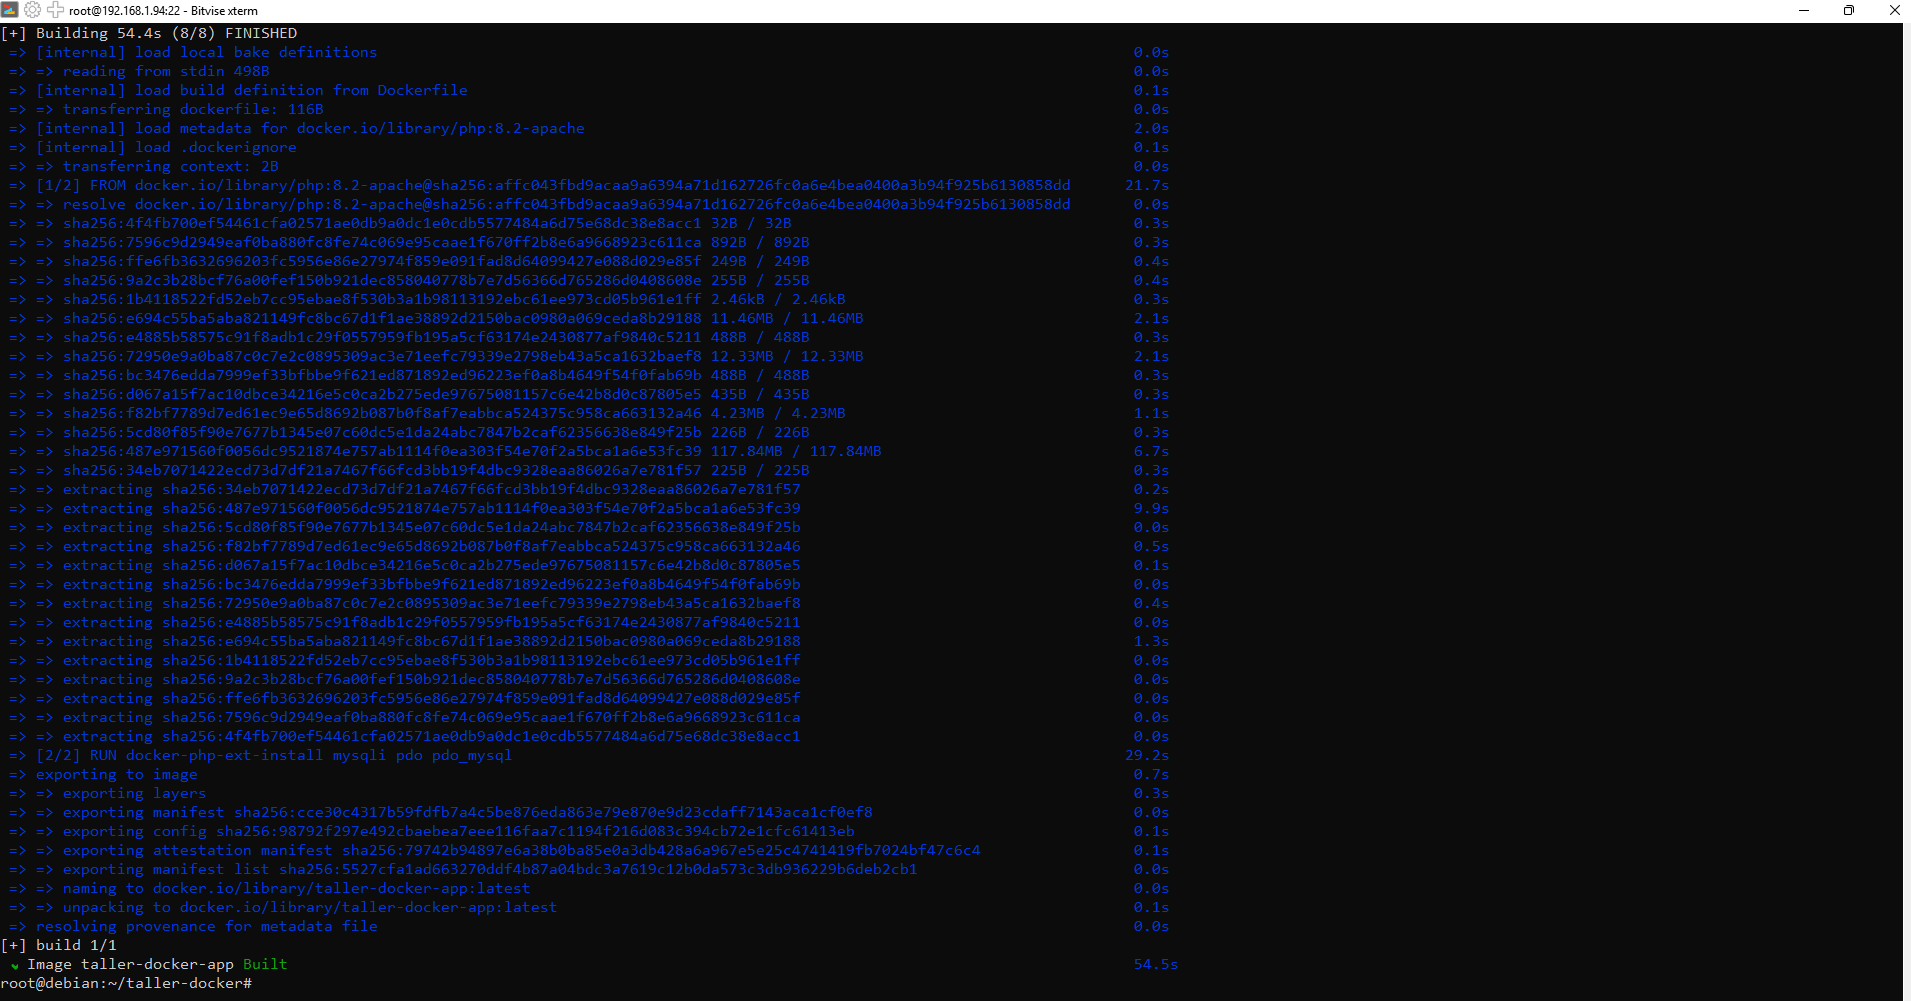
\includegraphics[width=0.9\textwidth]{images/BUILD.png}
    \caption{Proceso de construcción de la imagen app mediante Dockerfile.}
    \label{fig:build}
\end{figure}

\section{Ejecución}
Se utilizó el comando \texttt{docker compose up -d} para levantar los servicios en segundo plano, seguido del comando \texttt{docker ps}. La captura demuestra la correcta orquestación de la infraestructura, confirmando que tanto el contenedor de la aplicación web (mapeado al puerto local 8080) como el de la base de datos se encuentran en estado activo (Up) e interactuando en la red virtual \texttt{taller-red}.

\begin{figure}[H]
    \centering
    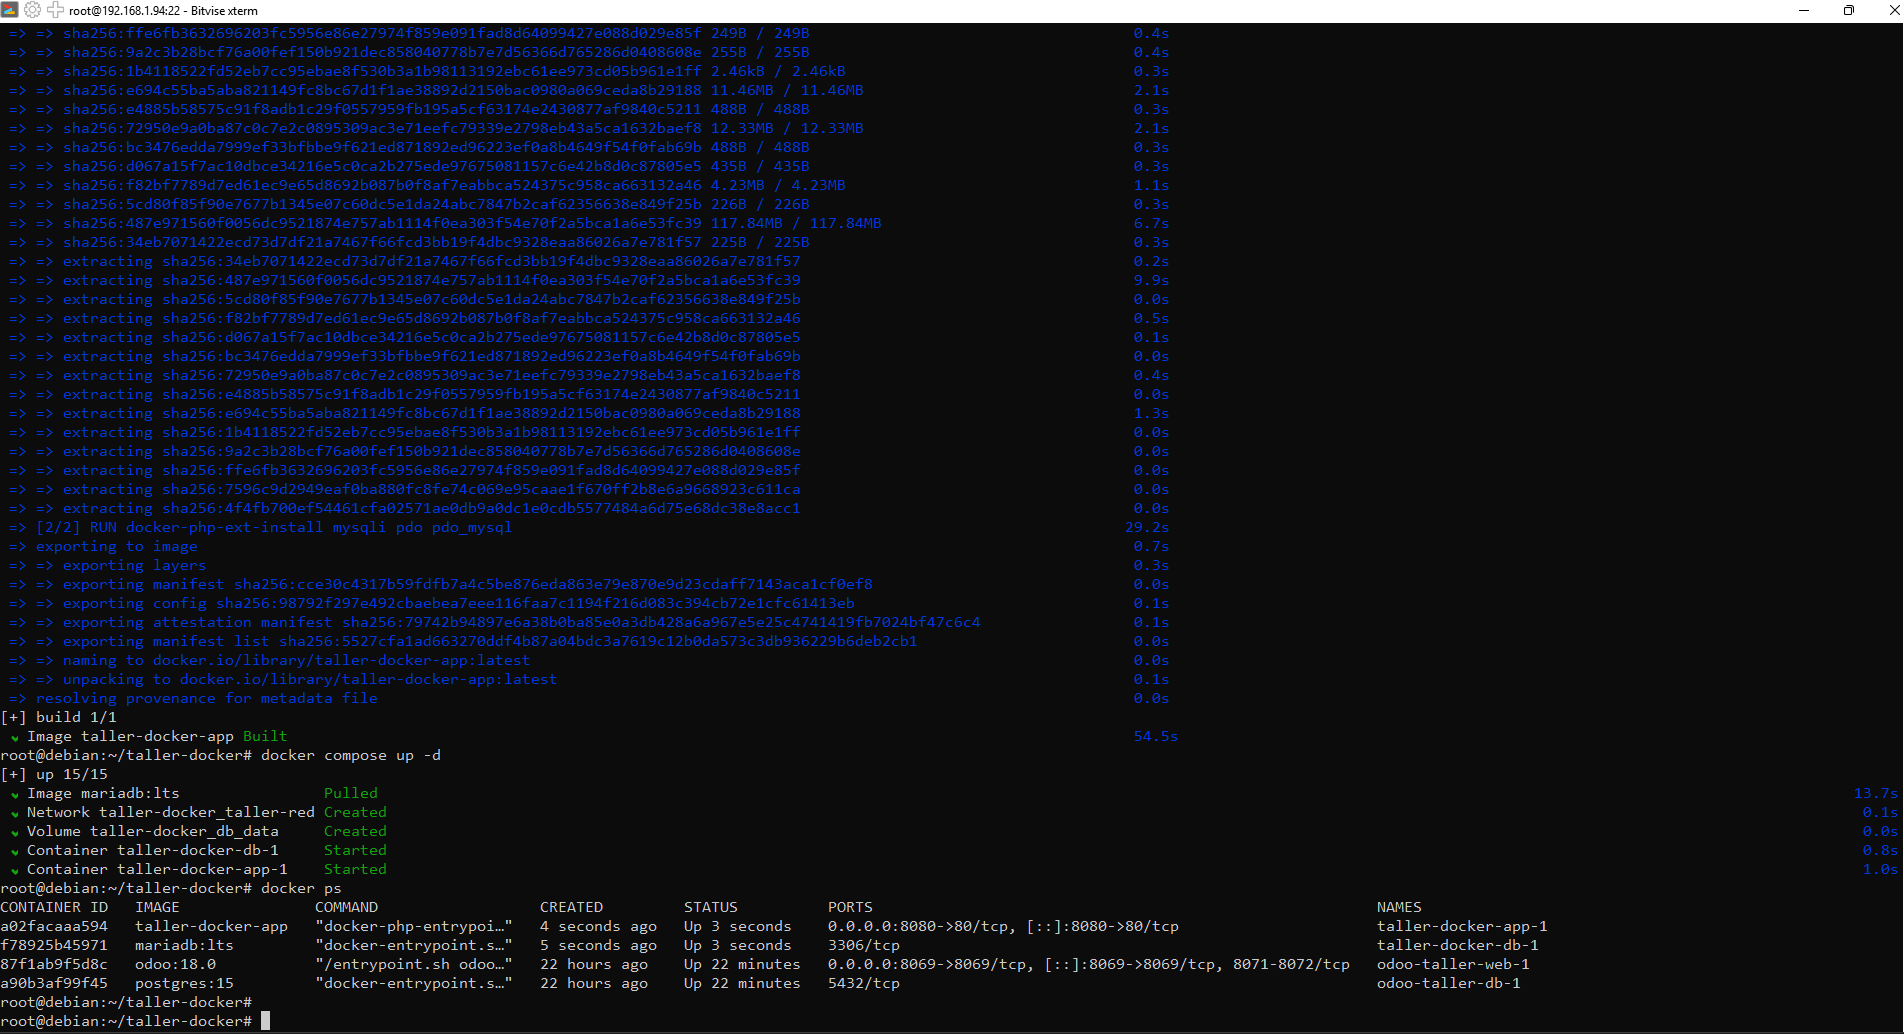
\includegraphics[width=0.9\textwidth]{images/CONTENEDORES TALLER-DOCKER Y MARIADB UP.png}
    \caption{Ejecución de contenedores y verificación de estado en la red.}
    \label{fig:ejecucion}
\end{figure}

\section{Logs/Red}
Para comprobar el correcto inicio del servicio MariaDB y la lectura del script de inicialización (\texttt{init.sql}), se inspeccionaron los registros mediante el comando \texttt{docker compose logs db}. La imagen verifica que el motor de base de datos se inicializó exitosamente, asignó los permisos correspondientes al usuario y se encuentra a la escucha de conexiones a través del puerto 3306 interno.

\begin{figure}[H]
    \centering
    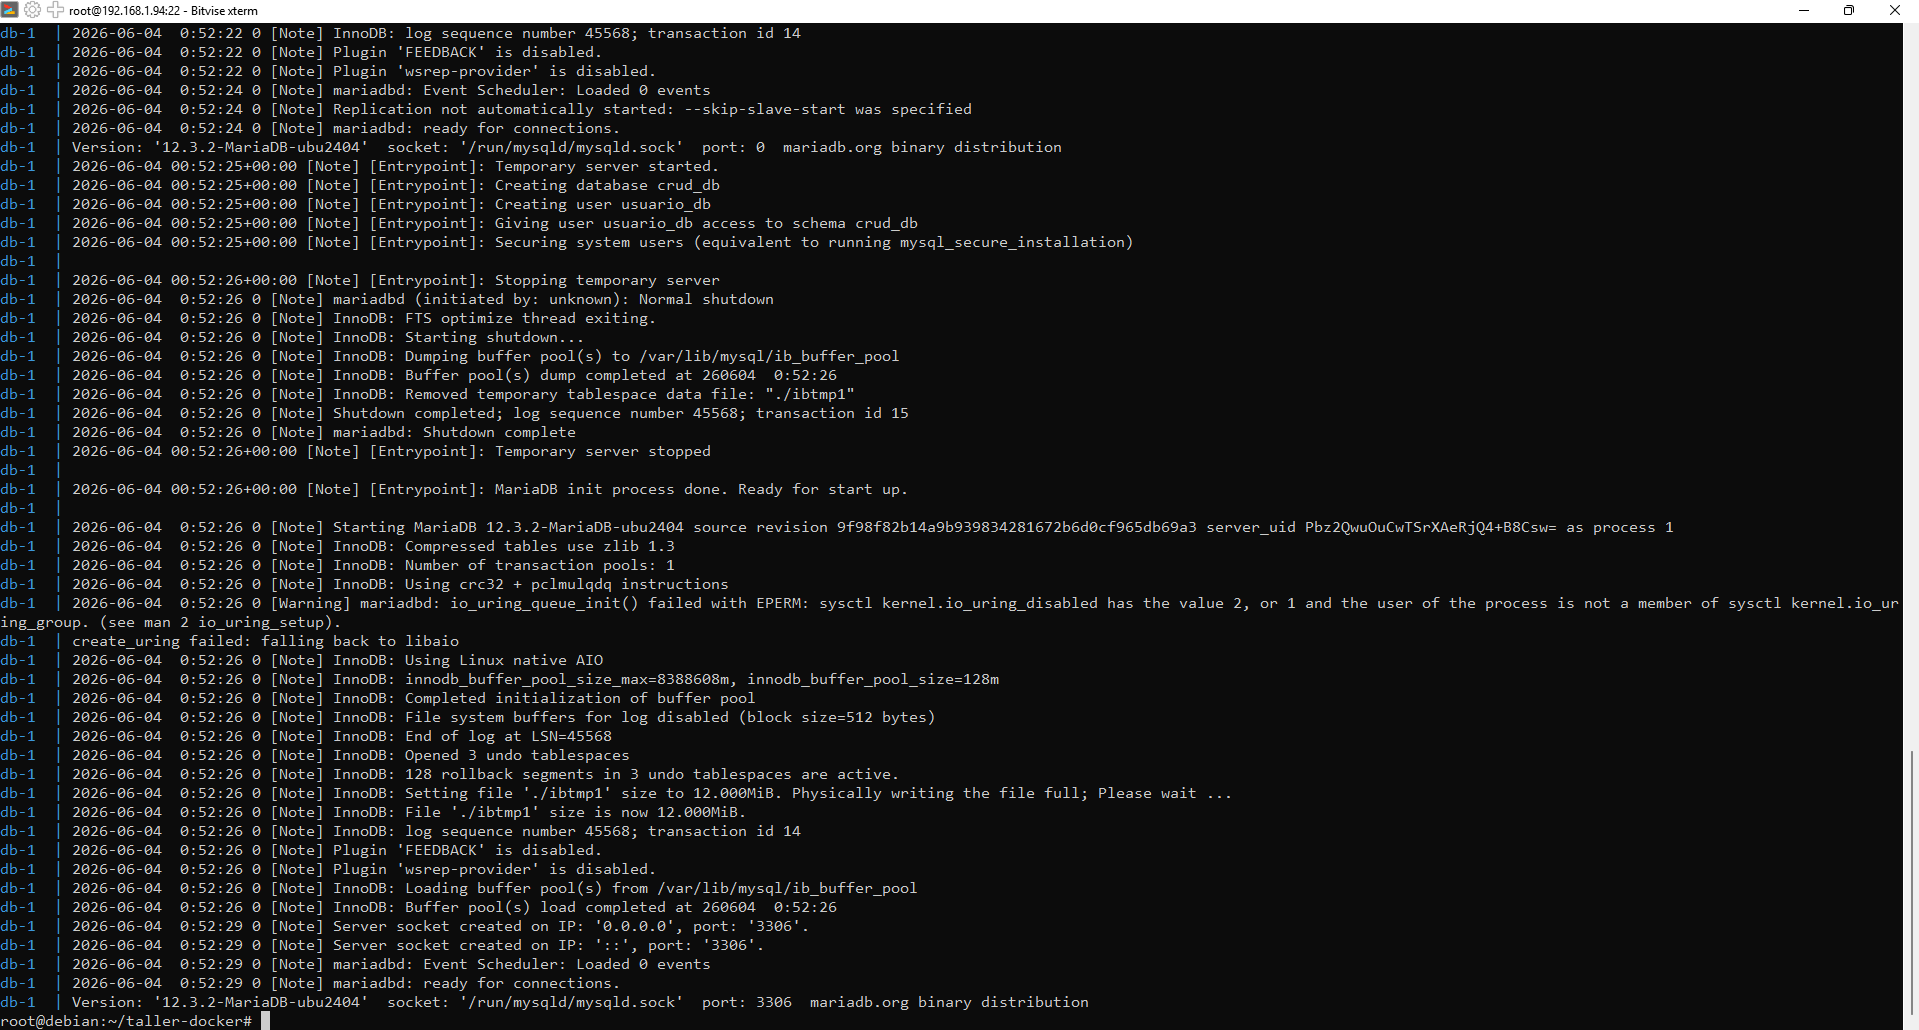
\includegraphics[width=1\textwidth]{images/MARIADB.png}
    \caption{Logs de inicio y configuración del contenedor MariaDB.}
    \label{fig:logs}
\end{figure}

\section{Prueba Funcional}
Finalmente, se accede a la aplicación web a través del navegador apuntando al puerto mapeado (8080). La captura demuestra la interfaz del menú principal cargando de manera óptima, conectada a la base de datos y lista para ejecutar la gestión de registros (CRUD) solicitada en los requisitos técnicos del laboratorio.

\begin{figure}[H]
    \centering
    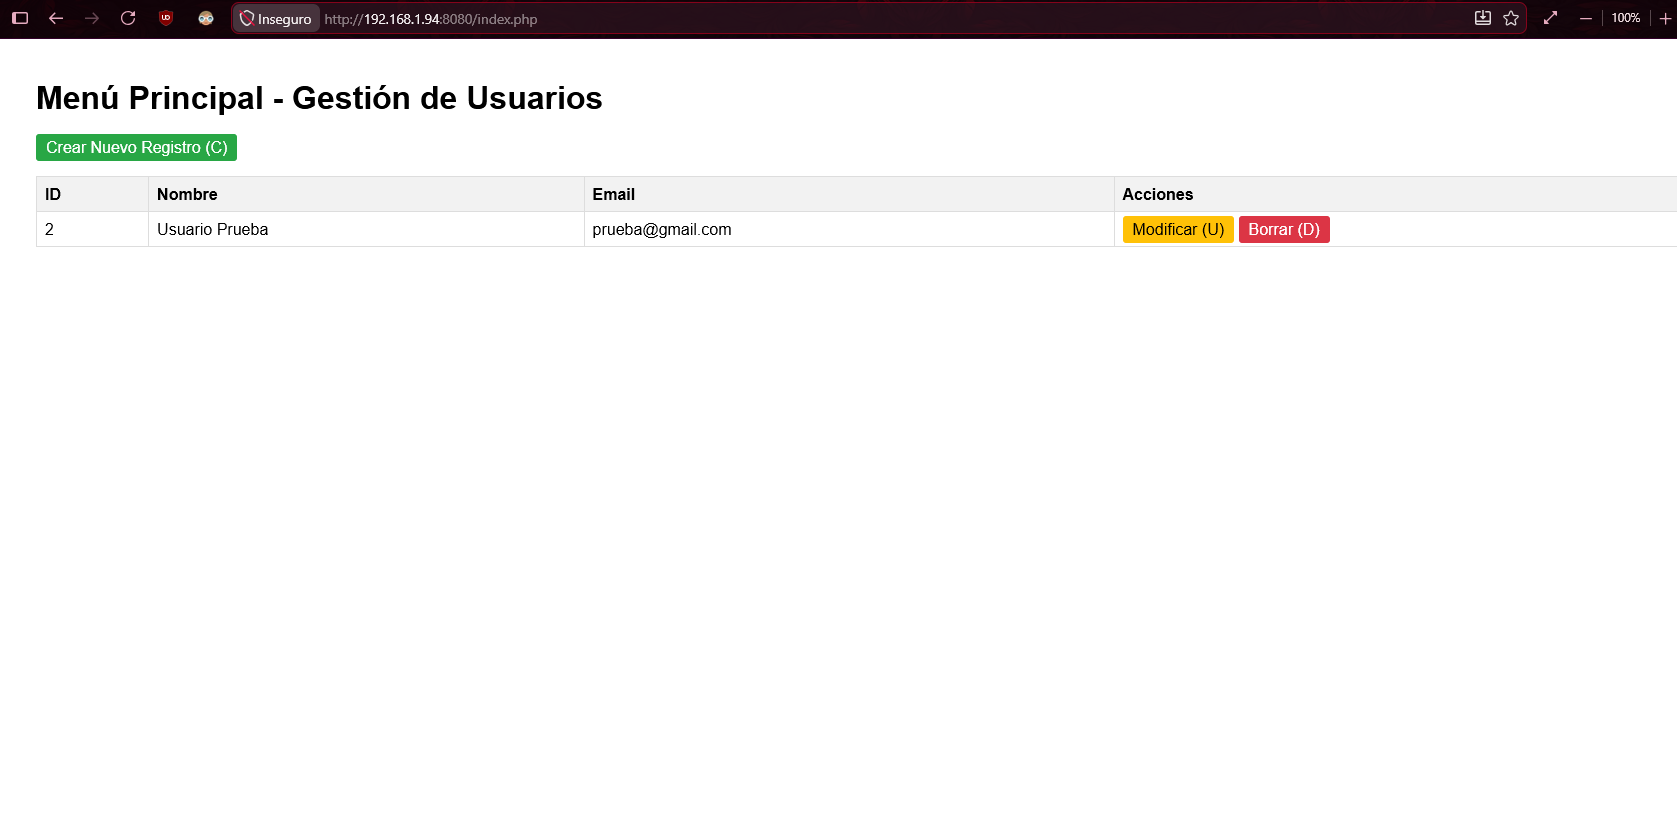
\includegraphics[width=1\textwidth]{images/index.png}
    \caption{Interfaz principal del CRUD mostrando los registros actuales.}
    \label{fig:index}
\end{figure}

\begin{figure}[H]
    \centering
    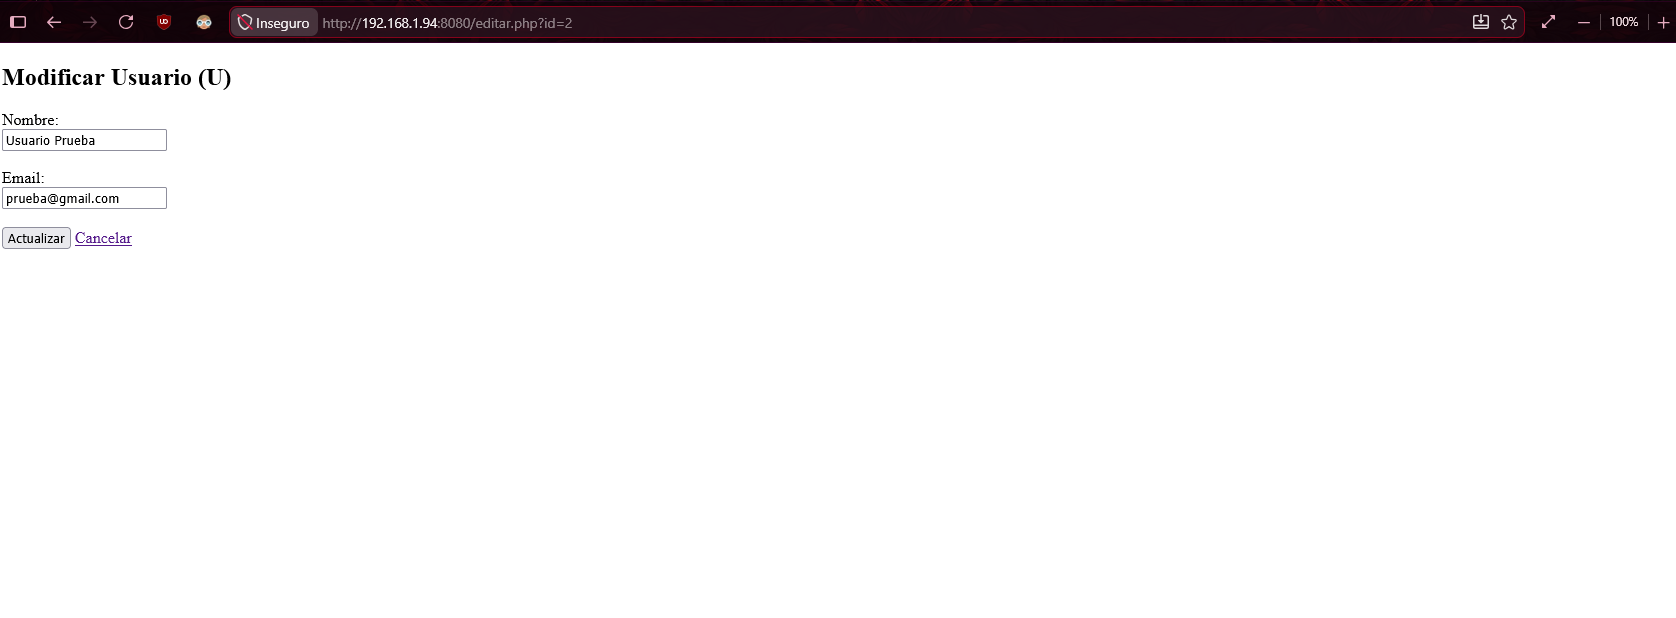
\includegraphics[width=1\textwidth]{images/editar.png}
    \caption{Formulario de actualización de datos de un registro existente.}
    \label{fig:editar}
\end{figure}

\begin{figure}[H]
    \centering
    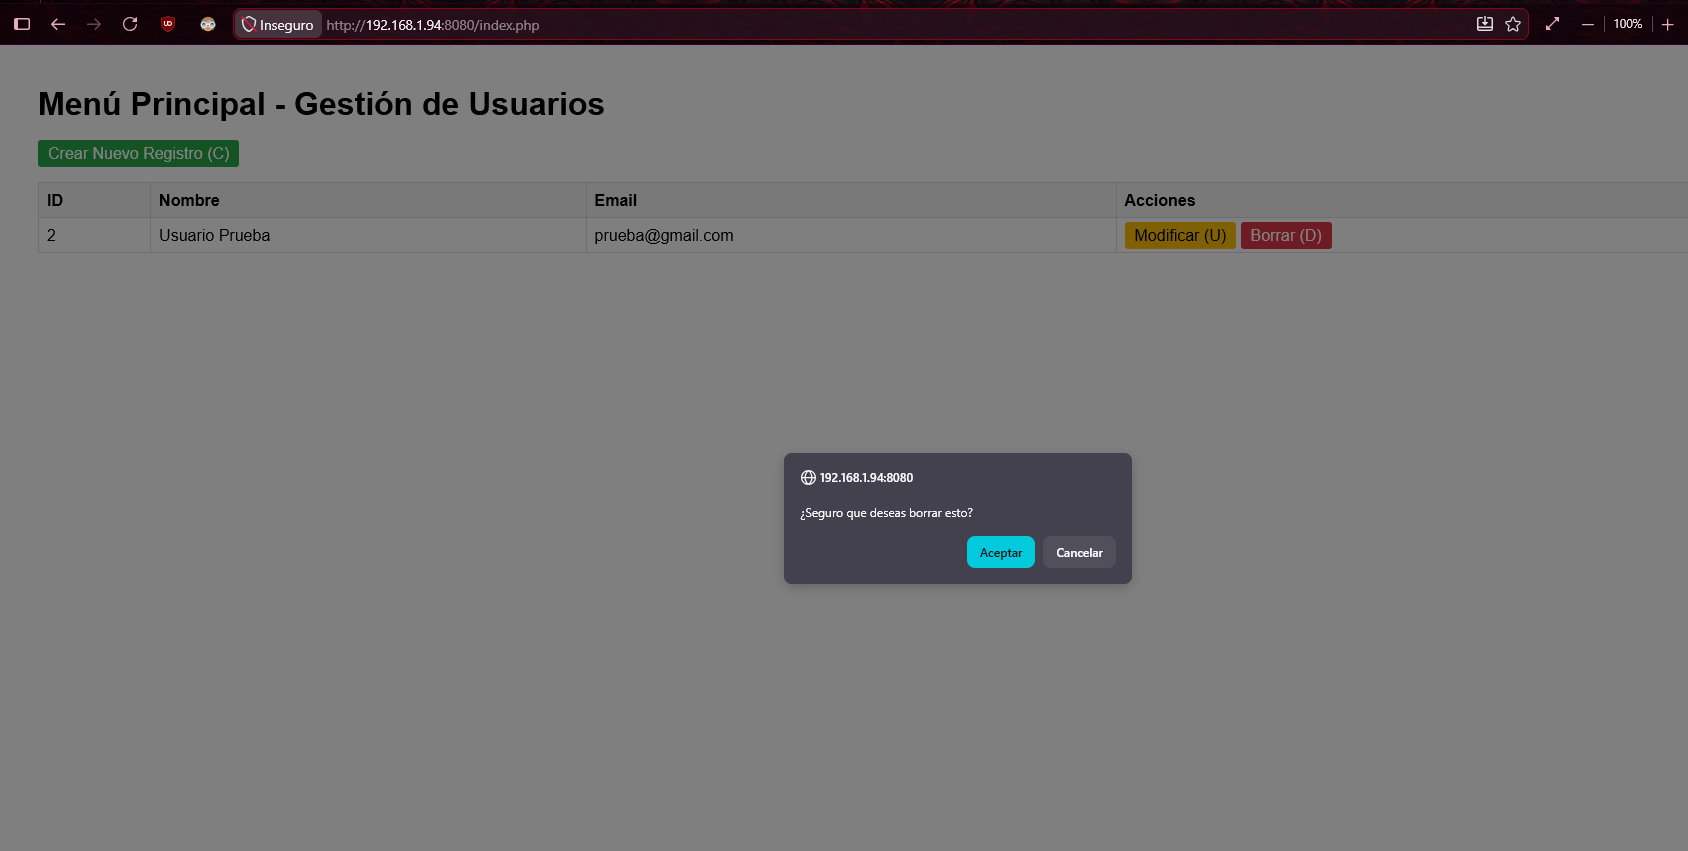
\includegraphics[width=1\textwidth]{images/borrar.png}
    \caption{Confirmación de eliminación de un registro en la base de datos.}
    \label{fig:borrar}
\end{figure}

\begin{figure}[H]
    \centering
    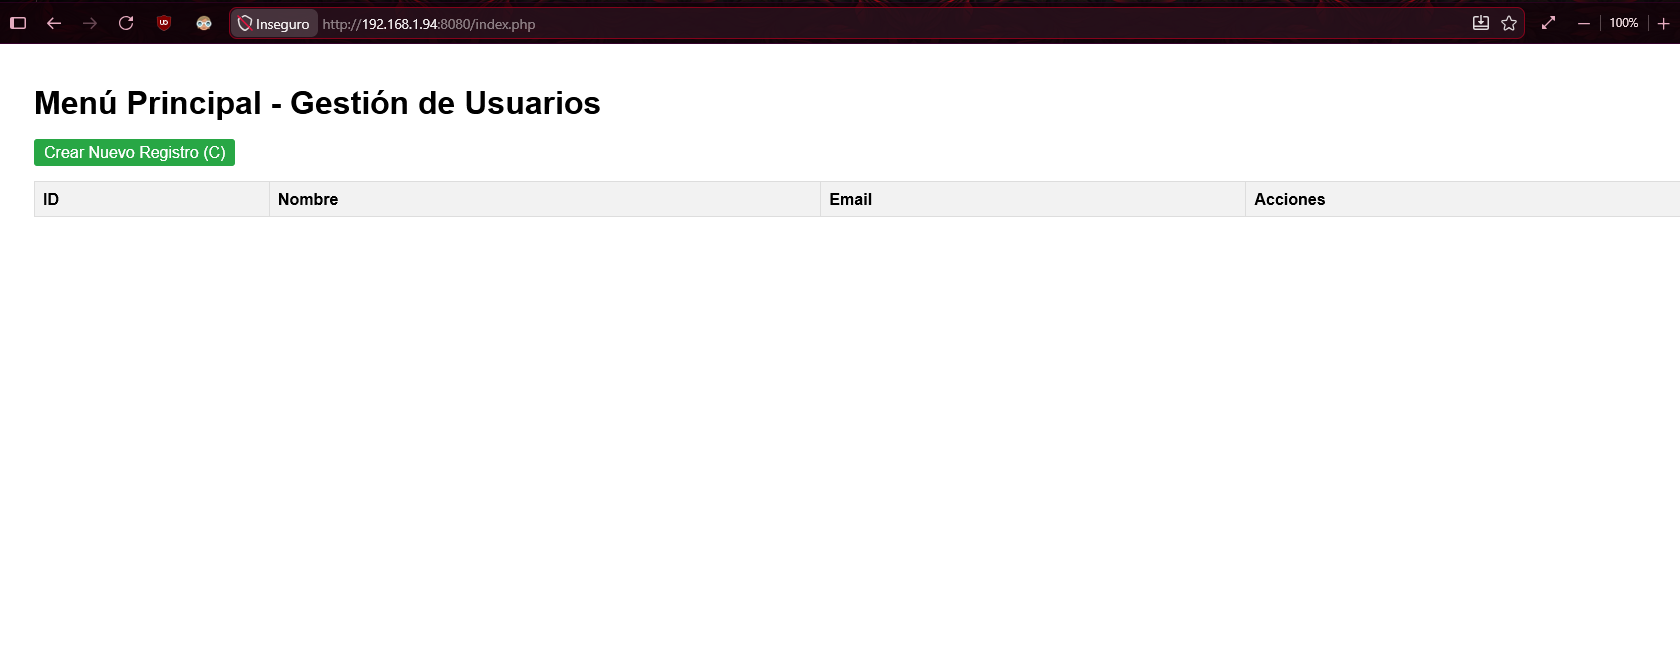
\includegraphics[width=1\textwidth]{images/todo limpio.png}
    \caption{Visualización de la tabla sin registros demostrando la limpieza total.}
    \label{fig:limpio}
\end{figure}

\chapter{Conclusión}

Un aspecto crítico evaluado fue la persistencia de datos. Mediante las asignaciones y configuraciones de volúmenes en Docker, se demostró directamente que la capa de datos mantiene su integridad de forma totalmente independiente a la volatilidad, detención o destrucción eventual de los contenedores. Esto demuestra el valor de abstraer el almacenamiento lógico del ciclo de vida del servicio, un estándar indispensable en entornos de producción reales. De igual forma, el aislamiento de los contenedores dentro de una red virtual privada (\texttt{taller-red}) permitió comprender cómo mitigar vectores de riesgo, limitando la exposición del motor de base de datos y forzando a que toda interacción ocurra de manera segura y exclusiva a través del servidor web\\
\\
Finalmente, el correcto funcionamiento de las cuatro operaciones fundamentales del sistema CRUD, evidenciado en la etapa de pruebas en el navegador, validó no solo la conectividad y resolución de nombres interna del stack, sino también la viabilidad de Docker como un ecosistema eficiente para el despliegue de aplicaciones. Los objetivos del laboratorio fueron alcanzados, dándole al equipo experiencia técnica esencial en infraestructura de programa, automatización y buenas prácticas de desarrollo modular.

\chapter{Anexos}
\section{Enlaces del Proyecto}
Todo el código fuente, la configuración de contenedores y los scripts de base de datos se encuentran respaldados con control de versiones. A continuación, se detallan los enlaces correspondientes:

\begin{itemize}
    \item \textbf{Repositorio en GitHub:} \url{https://github.com/KriegerN/taller-lab-2}
    \item \textbf{Link del documento en Overleaf:} \url{https://es.overleaf.com/read/jnknbppgxxdb#5aeb9d}
\end{itemize}

\section{Configuración Docker}
A continuación se detallan los archivos de configuración utilizados para la orquestación y construcción de los contenedores de este laboratorio.

\subsection{Archivo \texttt{docker-compose.yml}}
\begin{lstlisting}[frame=single, breaklines=true, basicstyle=\ttfamily\footnotesize]
services:
  app:
    build: ./app
    ports:
      - "8080:80"
    volumes:
      - ./app:/var/www/html
    networks:
      - taller-red
    depends_on:
      - db

  db:
    image: mariadb:lts
    restart: always
    environment:
      MYSQL_ROOT_PASSWORD: rootpassword
      MYSQL_DATABASE: crud_db
      MYSQL_USER: usuario_db
      MYSQL_PASSWORD: password_db
    volumes:
      - db_data:/var/lib/mysql
      - ./db/init.sql:/docker-entrypoint-initdb.d/init.sql
    networks:
      - taller-red

networks:
  taller-red:
    driver: bridge

volumes:
  db_data:
\end{lstlisting}

\subsection{Archivo \texttt{Dockerfile}}
\begin{lstlisting}[frame=single, breaklines=true, basicstyle=\ttfamily\footnotesize]
FROM php:8.2-apache
RUN docker-php-ext-install mysqli pdo pdo_mysql
EXPOSE 80
\end{lstlisting}